% !TEX TS-program = pdflatex
% !TEX encoding = UTF-8 Unicode

% This is a simple template for a LaTeX document using the "article" class.
% See "book", "report", "letter" for other types of document.

\documentclass[11pt]{article} % use larger type; default would be 10pt
\usepackage{multirow}
\usepackage[utf8]{inputenc} % set input encoding (not needed with XeLaTeX)
%%% Examples of Article customizations
% These packages are optional, depending whether you want the features they provide.
% See the LaTeX Companion or other references for full information.
\usepackage[czech]{babel}
%%% PAGE DIMENSIONS
\usepackage{geometry} % to change the page dimensions
\geometry{a4paper} % or letterpaper (US) or a5paper or....
\geometry{margin=0.5in} % for example, change the margins to 2 inches all round
% \geometry{landscape} % set up the page for landscape
%   read geometry.pdf for detailed page layout information

\usepackage{graphicx} % support the \includegraphics command and options
\usepackage{tabularx}
\usepackage{wrapfig}
\usepackage{hyperref}
% \usepackage[parfill]{parskip} % Activate to begin paragraphs with an empty line rather than an indent

%%% PACKAGES
\usepackage{booktabs} % for much better looking tables
\usepackage{array} % for better arrays (eg matrices) in maths
\usepackage{paralist} % very flexible & customisable lists (eg. enumerate/itemize, etc.)
\usepackage{verbatim} % adds environment for commenting out blocks of text & for better verbatim
\usepackage{subfig} % make it possible to include more than one captioned figure/table in a single float
% These packages are all incorporated in the memoir class to one degree or another...

%%% HEADERS & FOOTERS
\usepackage{fancyhdr} % This should be set AFTER setting up the page geometry
\pagestyle{fancy} % options: empty , plain , fancy
\renewcommand{\headrulewidth}{0pt} % customise the layout...
\lhead{}\chead{}\rhead{}
\lfoot{}\cfoot{\thepage}\rfoot{}

%%% SECTION TITLE APPEARANCE
\usepackage{sectsty}
\allsectionsfont{\sffamily\mdseries\upshape} % (See the fntguide.pdf for font help)
% (This matches ConTeXt defaults)

%%% ToC (table of contents) APPEARANCE
\usepackage[nottoc,notlof,notlot]{tocbibind} % Put the bibliography in the ToC
\usepackage[titles,subfigure]{tocloft} % Alter the style of the Table of Contents
\renewcommand{\cftsecfont}{\rmfamily\mdseries\upshape}
\renewcommand{\cftsecpagefont}{\rmfamily\mdseries\upshape} % No bold!

%%% END Article customizations

%%% The "real" document content comes below...

\title{Zápočtový program - FFT ekvalizér}
\author{Petr Martišek}
\date{} % Activate to display a given date or no date (if empty),
         % otherwise the current date is printed 

\begin{document}
\maketitle

\section{Anotace}
Cílem zápočtové práce bylo implementovat jednoduchý pásmový ekvalizér za použití algoritmu FFT. Program umí pracovat pouze s jednoduchými *.wav soubory bez jakékoliv komprese.

\section{Interface}
Program je spouštěn z příkazové řádky s následujícími parametry:
\vskip 10 pt
\texttt{ffteq \emph{INPUT\_FILE} [-o \emph{OUTPUT\_FILE}] [-e \emph{LOWER\_BOUND UPPER\_BOUND QUOTIENT}] [-e \ldots] \ldots}
\vskip 10 pt
\noindent Argument \texttt{\emph{INPUT\_FILE}} je povinný a definuje cestu ke vstupnímu souboru. Ten musí být ve formátu RIFF WAV s PCM kódováním, tj. bez jakékoliv komprese. Soubor v jiném formátu program odmítne.

Nepovinný přepínač \texttt{-o} s parametrem \texttt{\emph{OUTPUT\_FILE}} definuje cestu k výstupnímu souboru. Není-li výstupní soubor definován, vytvoří se automaticky se jménem odvozeným od vstupního (konkrétně \texttt{\emph{INPUT\_FILE}\_eq.wav}).

Přepínač \texttt{-e} se třemi parametry definuje samotnou ekvalizaci. První dva parametry, \texttt{\emph{LOWER\_BOUND}}\\ a \texttt{\emph{UPPER\_BOUND}}, udávají dolní a horní hranici frekvenčního pásma v Hertzích, na které se má ekvalizace aplikovat. Třetí parametr \texttt{\emph{QUOTIENT}} udává procento změny. Např. kvocient 0.5 způsobí ztlumení daného frekvenčního pásma na 50~\%, kvocient 2.0 jej naopak zesílí na dvojnásobek. Ekvalizací lze aplikovat libovolné množství opakovaným použitím argumentu \texttt{-e}. Je-li na nějakou oblast spektra aplikováno postupně více ekvalizací, efekty se sčítají.

Přepínač \texttt{-h} zobrazí nápovědu a ukončí program (nehledě na případné ostatní argumenty).

Příklad korektního volání programu:
\vskip 10 pt
\texttt{ffteq input.wav -o output.wav -e 20 500 0.3 -e 14000 22000 2.3}
\vskip 10 pt
Tato konfigurace způsobí ztlumení frekvencí v pásmu 20 až 500~Hz na 30~\% a současně zesílení frekvencí v~pásmu 14~kHz až 22~kHz na 230~\%.

Dlužno podotknout, že rozsah frekvencí, na něž lze ekvalizaci aplikovat, je shora omezen $\frac{F_S}{2}$, kde $F_S$ je vzorovací frekvence vstupního souboru (typicky 44,1~kHz). Toto plyne z Shannon-Nyquistova teorému a tato hraniční frekvence se nazývá Nyquistova. Vyšší frekvence na vstupu budou automaticky seříznuty na tuto hodnotu.

\section{Program}
\subsection{Parsování vstupu}
Snad netřeba podrobnějšího vysvětlování. Parsování argumentů, uložení ekvalizačních parametrů do vektoru trojic \texttt{eqParam}, který později předáme modifikační funkci.

\subsection{Přečtení a naparsování vstupního souboru}
V další části otevřeme vstupní soubor a celý jej překopírujeme po bytech do bufferu -- což je pole s prvky typu \texttt{char}. Postupně přečteme hlavičku a informace si ukládáme do vlastních proměnných. \emph{(Pro vysvětlení struktury *.wav souboru viz. Příloha.)} Následně přečteme samotná data a uložíme je do vektorů \texttt{channels} odpovídajících jednotlivým kanálům. Počet těchto kanálů je odvozen od hodnoty \texttt{NumChannels}. Velikost vzorků, které \uv{ukrajujeme} z bufferu, odpovídá hodnotě \texttt{BitsPerSample}. Technicky je toho dosaženo použitím funkce \texttt{reinterpret\_cast}, kdy přetypujeme ukazatel do bufferu z \texttt{char*} na \texttt{signed short*} nebo \texttt{signed long*} -- podle počtu bytů, které chceme uříznout -- a následně cíl tohoto ukazatele překopírujeme do vlastního vektoru.

Vzorky jsou v souboru setříděny podle času, nikoli podle kanálu. To znamená, že vzorky pro všechny kanály pro nějaký daný čas jsou u sebe, v jednom bloku.

Program je schopen zpracovat soubory vzorkované až do hloubky 32 bitů, což je pro běžné potřeby dostačující (CD kvalita je 16 bitů). Vyšší hodnoty se používají pouze např. při profesionálním zpracování audia v hudebních studiích.

\subsection{Fourierova transformace}
Samotný algoritmus transformace je implementován ve třídě \texttt{Fft}. Jedná se o nerekurzivní in-place algoritmus o složitosti $\Theta(n \log n)$. Každý kanál budeme zpracovávat zvlášť, vytvoříme tedy instatnci třídy \texttt{Fft} pro každý z nich. Konstruktoru předáme jako parametr nejnižší mocninu dvojky vyšší než počet vzorků. Při vzniku instance třídy dojde k dvěma výpočtům. Prvním je předpočítání mapy pro bitově reverzní setřídění vzorků, což je nezbytný krok pro implementaci efektivní in-place varianty. Toho je dosaženo vhodným přepínáním bitů pomocí bitové masky. Druhým krokem je výpočet mocnin primitivní n-té odmocniny z jedné, které jsou třeba v chodu algoritmu. Předpočteme hodnoty pro všechny úrovně algoritmu. Pro inverzní transformaci s výhodou použijeme tytéž hodnoty, jen komplexně sdružené.

Pomocí metody \texttt{CopyIn} překopírujeme do instance třídy vektor vzorků získaných z *.wav souboru, přičemž je však do in-place bufferu ukládáme již v reverzně-bitově setříděném pořadí, a to pomocí předpočítané mapy.

Následně v každém kanálu proběhne samotná FFT, čímž se prvky in-place bufferu změní na reprezentaci frekvenčního spektra daného kanálu. Implementace klíčového jádra algoritmu je díky předvýpočtům již poměrně jednoduchá. Při pohledu na grafické znázornění průběhu výpočtu FFT pomocí hradlové sítě (tzv. \emph{butterfly} výpočet) by měl být význam jednotlivých kroků a proměnných v kódu zřejmý.
\subsection{Ekvalizace}
Ekvalizace je realizována metodou \texttt{Equalize}, které jsou předány jako parametry vzorkovací frekvence a ekvalizační předpisy ve formátu vektoru trojic \emph{(dolní\_frekvence, horní\_frekvence, kvocient)}. 

Pro správnou aplikaci ekvalizace je nejprve třeba správně interpretovat výstup FFT. Pro vstupní vektor $n$ reálných čísel je výstupem vektor $n$ komplexních čísel, kde reálná část reprezentuje koeficienty funkce $cos$ odpovídající frekvence a imaginární reprezentuje funkci $sin$. Výpočet frekvence, která je komplexním číslem na daném indexu reprezentována, je následující:
$$frequency = \frac{index \times SampleRate}{n}$$
Např. pro vzorkovací frekvenci 44,1~kHz a počet vzorků 1024 je interpretace následující:
\begin{enumerate}
\leftskip 180 pt
\setcounter{enumi}{-1}
\item  $0 \times 44100 / 1024 = 0,0$~Hz
\item  $1 \times 44100 / 1024 = 43,1$~Hz
\item  $2 \times 44100 / 1024 = 86,1$~Hz \\
\ldots
\setcounter{enumi}{511}
\item  $512 \times 44100 / 1024 = 22050,0$~Hz
\end{enumerate}

Pro reálný vstup je druhá polovina výsledku FFT jen komplexně sdruženým obrazem první poloviny a tedy neobsahuje informace o žádných dalších frekvencích. Více viz \cite{fftguru} (kapitola 6). Nejvyšší detekovaná frekvence se nachází na indexu $n/2$ a jedná se o již zmíněnou Nyquistovu frekvenci.

V praxi to znamená dvě věci: Jednak musíme pohlídat, že parametry ekvalizace zadané uživatelem jsou v~rozumných mezích (tedy větší než nula a menší nebo rovny Nyquistově frekvenci) a jednak musíme vynulovat hodnoty v druhé polovině výsledku FFT, což současně vykompenzujeme zdvojnásobením intenzity hodnot v~první polovině. Teoreticky bychom mohli nechat spektrum nezměněné a výsledek bude stejný, ale v praxi to může vést ke vzniku šumu a různých artefaktů. Takto těmto nepříjemnostem zabráníme a současně nedojde ke ztrátě informace.
\subsection{Inverzní transformace}
Po aplikaci ekvalizace je třeba provést inverzní transformaci. Její implementace se od dopředné liší ve třech detailech. Zaprvé je třeba in-place buffer, který nyní obsahuje frekvenční spektrum, opět bitově reverzně setřídit. To nutně vede k překopírování dat do dalšího vektoru a abychom si ušetřili další kopírování, provedeme samotnou transformaci v tomto novém bufferu. Druhým rozdílem je použití komplexně sdružených obrazů předpočtených exponenciál. Posledním detailem je normalizace výsledku, tj. vydělení všech prvků ve výsledném vektoru velikostí tohoto vektoru. Přitom si rovnou výsledek překopírujeme zpět do původního in-place bufferu.
\subsection{Výstup}
Pro každý kanál získáme výsledek z instance třídy \texttt{Fft} pomocí metody \texttt{GetResult}. Což je vektor komplexních čísel. Ten přetypujeme na správný typ (podle proměnné \texttt{BitsPerSample}) a po překopírování hlavičky jej zapíšeme do výstupního souboru. Opět postupujeme podle času, tedy zapíšeme hodnotu pro daný index pro všechny kanály a až pak se přesuneme na další index. Při zapisování vzorků vetších než 1 byte musíme vzít v~úvahu i kódování, konkrétně je třeba převést vzorky z Big Endian na Little Endian. Pomocí bitové masky a~bitového posunu to však není žádný větší problém.

\section*{Příloha: Formát *.wav souboru}
Pro práci s *.wav soubory je samozřejmě nutné znát jejich strukturu. Ta je ukázána na následující grafice\cite{wavspec}:
\begin{minipage}[c]{\textwidth}
\begin{center}
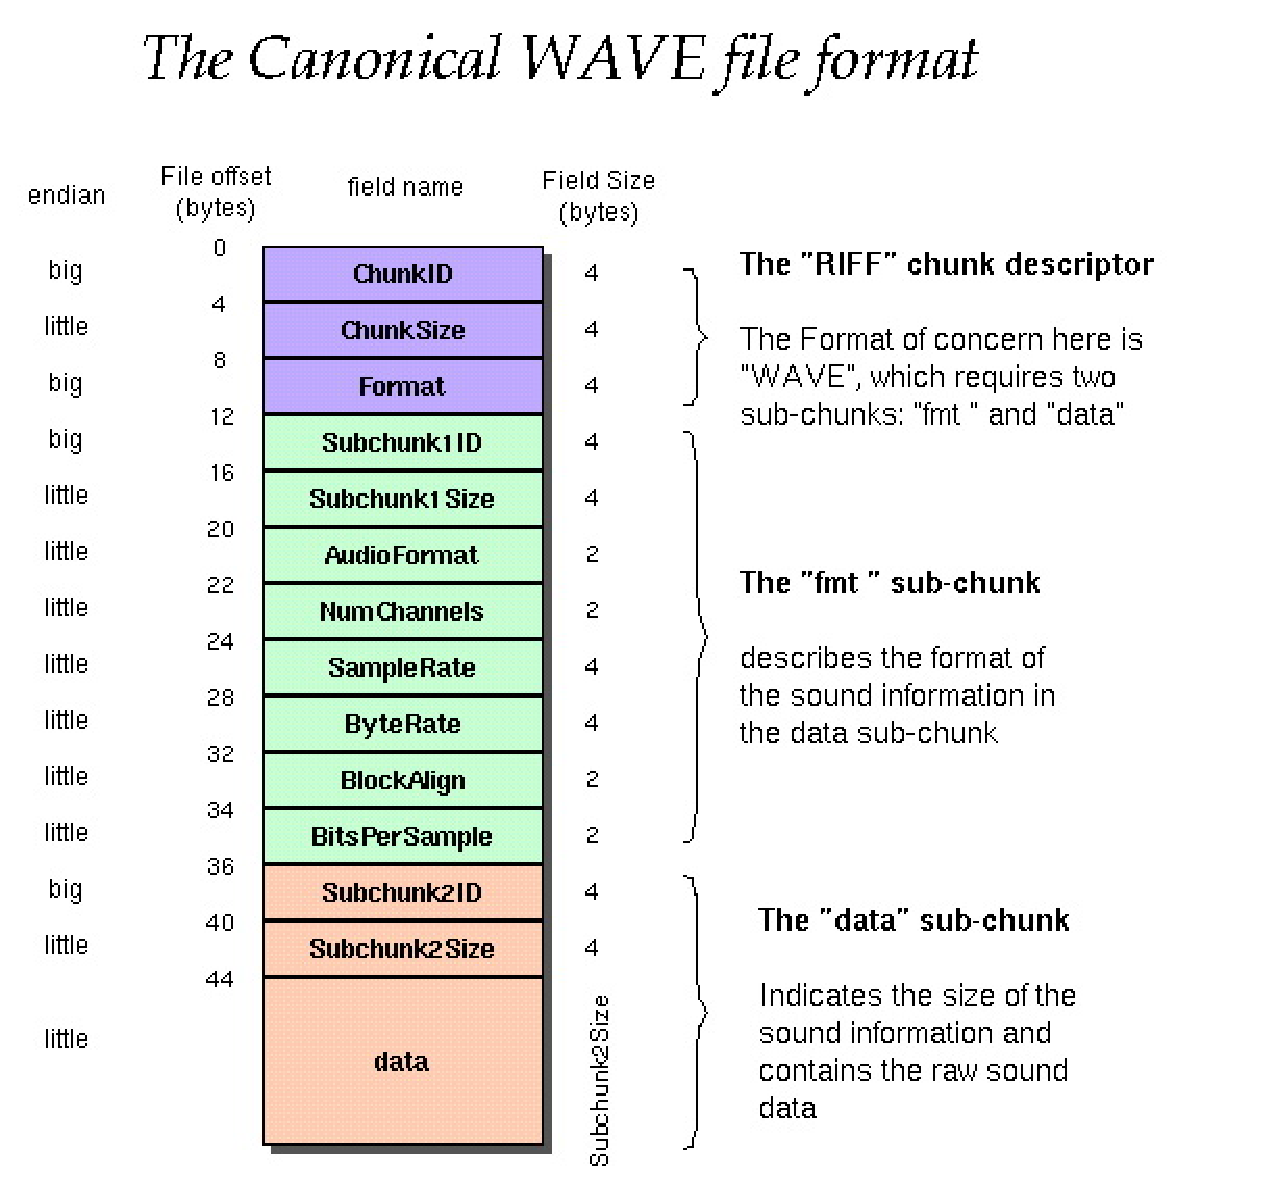
\includegraphics[scale=0.5]{wav-sound-format.pdf}
\end{center}
\end{minipage}
\renewcommand{\arraystretch}{1.2}
\begin{tabularx}{\textwidth}{| l| X |}
\hline
 ChunkID & Obsahuje slovo \uv{RIFF} v ASCII kódu.\\
\hline
 ChunkSize & Velikost zbytku souboru po tomto poli, tj. faktická velikost souboru mínus 8.\\
\hline
 Format & Obsahuje slovo \uv{WAVE} v ASCII kódu. \\
\hline
 Subchunk1ID &  Obsahuje slovo \uv{fmt } v ASCII kódu.\\
\hline
 Subchunk1Size & 16 pro PCM. Velikost zbytku sekce \uv{fmt}.\\
\hline
 AudioFormat & 1 pro PCM. Jiná hodnota znamená nějakou kompresi.\\
\hline
\textbf{NumChannels }& \textbf{Mono = 1, Stereo = 2, atd.}\\
\hline
\textbf{SampleRate} & \textbf{8000, 44100, atd}.\\
\hline
 ByteRate & $SampleRate \times NumChannels \times BitsPerSample/8$\\
\hline
 BlockAlign & $NumChannels \times BitsPerSample/8$\\
\hline
\textbf{BitsPerSample} & \textbf{8 bits = 8, 16 bits = 16, atd.}\\
\hline
 Subchunk2ID & Obsahuje slovo \uv{data} v ASCII kódu.\\
\hline
 Subchunk2Size & $NumSamples \times NumChannels \times BitsPerSample/8$. Velikost zbytku této sekce (tj. fakticky velikost vlastních zvukových dat).\\
\hline
Data & Samotná data.\\
\hline
\end{tabularx}
\begin{thebibliography}{9}

\bibitem{fftguru}
Kevin J. McGee,
\emph{An Introduction to Signal Processing and Fast Fourier Transform (FFT) (excerpt)},
2009,
\url{http://fftguru.com/fftguru.com.tutorial.pdf}
\ Vynikající materiál o Fourierově transformaci, cenným zdrojem byla zejména pasáž o interpretaci výsledků a záporných frekvencích.
\bibitem{wavspec}
\url{https://ccrma.stanford.edu/courses/422/projects/WaveFormat/}
  Přehledný rozbor struktury standardního *.wav souboru.
\end{thebibliography}
\end{document}
